\chapter{Adquisición de datos}

Esta clase tiene como objetivo comprender los pasos básicos para adquirir imágenes satelitales. Para ello se descargarán imágenes de la web del USGS y se procesarán para poder ser utilizadas en el SNAP.

\section{Descarga de imágenes}

Para descargar imágenes utilizaremos el catálogo del \href{https://earthexplorer.usgs.gov/}{USGS}\footnote{\href{https://earthexplorer.usgs.gov/}{https://earthexplorer.usgs.gov/}}. Para utilizarlo deberá registrarse en el sitio web. Diríjase luego a la página y en la pestaña \texttt{Seach Criteria} seleccione \texttt{Address/Place} y escriba \texttt{Iguazú} haciendo luego click en \menu{Show} (Figura \ref{fig:busqueda}).

\begin{figure}[h!]
    \centering
    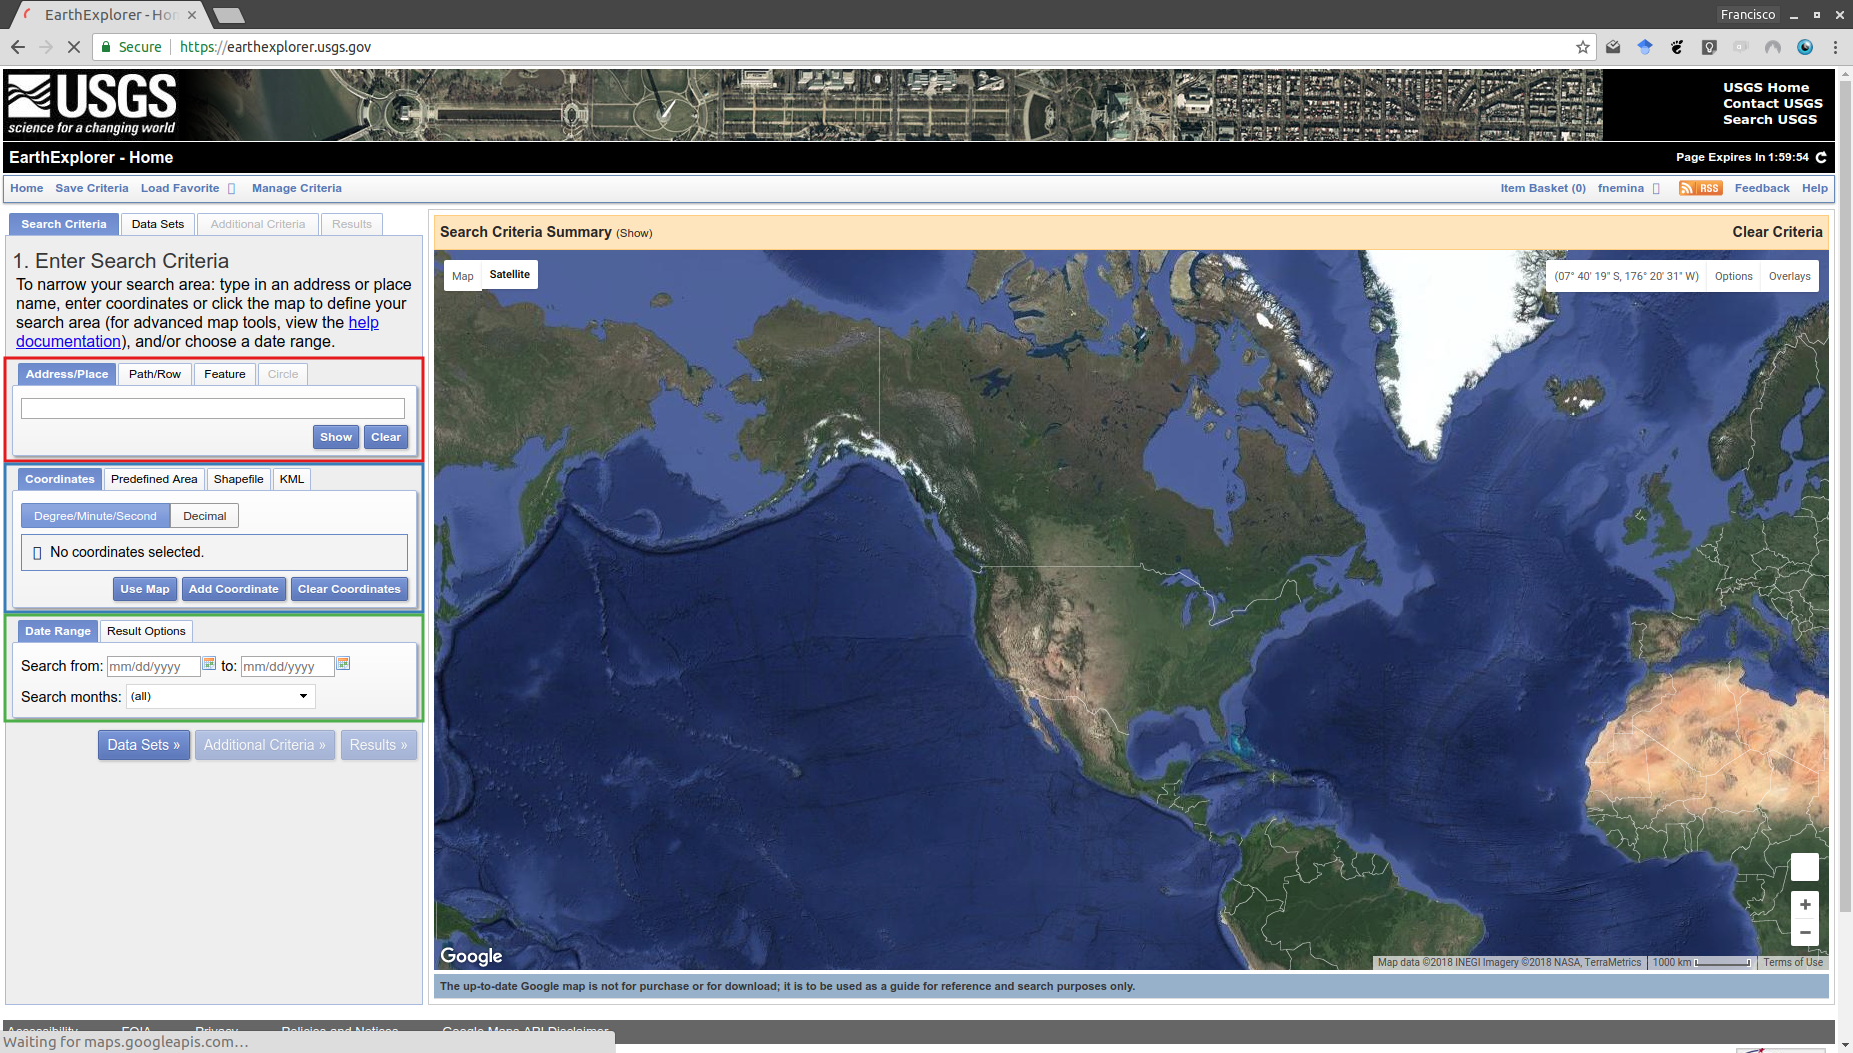
\includegraphics[width=0.6\textwidth]{fig:busqueda.png}
    \caption{Busqueda en el catálogo del \emph{USGS}. Puede observarse el área de busqueda en rojo, el área seleccionada en azul y la selección temporal en verde.}
    \label{fig:busqueda}
\end{figure}

Luego haga click sobre el nombre \texttt{Misiones Province, Argentina} para seleccionar dicha zona en el mapa. Seleccione luego en \menu{Data Range} las fechas 1 de julio de 2017 y 31 de julio de 2017.

Haga click en \menu{Data Sets} y en el cuadro \texttt{Data Set Search:} escriba \texttt{Landsat 8} y seleccione del menú la opción \texttt{Landsat 8 OLI/TIRS C1 Level-2} (Figura \ref{fig:dataset}) para seleccionarlo. Haga luego click en \menu{Results}.

\begin{figure}[h!]
    \centering
    
\includegraphics[width=0.6\textwidth]{fig:dataset.png}
    \caption{Selección de un set de datos en el catálogo del \emph{USGS}. Puede observarse el área de busqueda en rojo y los set de datos seleccionados tildados dentro del recuadro verde.}
    \label{fig:dataset}
\end{figure}

A la izquierda de la pantalla aparecerá una lista de productos. Busque entre ellos al correspondiente al 13 de julio del 2017, del path 224 y el row 78. Haga click sobre \menu{Order scene} (Figura \ref{fig:descarga}).

\begin{figure}[H]
    \centering
    \subfloat[]{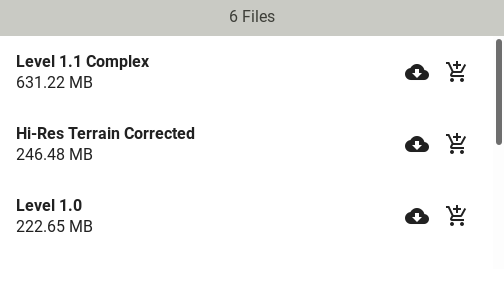
\includegraphics[width=0.6\textwidth]{fig:descarga.png}}
    \\
    \subfloat[]{
\includegraphics[scale=0.5]{fig:operaciones.png}}
    \caption{a) Selección de producto para la descarga en el catálogo \emph{Vertex} del \emph{USGS}. En rojo el botón para ver el pedido. b)Herramientas del catálogo. De izquierda a derecha se observa: Footprint, Show Browse Overlay, Compare Browse, Show Metadata and Brose, Order Scene y Exlude escene from Results.}
    \label{fig:descarga}
\end{figure}

Para corroborar el pedido haga click en \menu{View Item Basket} y luego en \menu{Proceed to Checkout}. Finalmente deberá solicitar la imagen haciendo click en \menu{Submit Order}.

El producto descargado pertenece a una serie de productos a demanda.  Cuando  esté disponible para descargar se le enviará un correo electrónico notificandolo \footnote{Recibirá 3 correos electrónicos en total: dos confirmando el pedido y uno cuando la descarga esté disponible}. El asunto será

\begin{center}
\texttt{USGS ESPA product request order number [] available for download}
\end{center}

con \texttt{[]} el número de pedido. Haga click en el link dentro del correo y en la página que se abre seleccione su pedido en la columna \texttt{Order ID}. Finalmente haga click en \texttt{Download} en la columna \texttt{Product URL} para descargar la imagen.

\begin{figure}[h!]
    \centering
    \subfloat[]{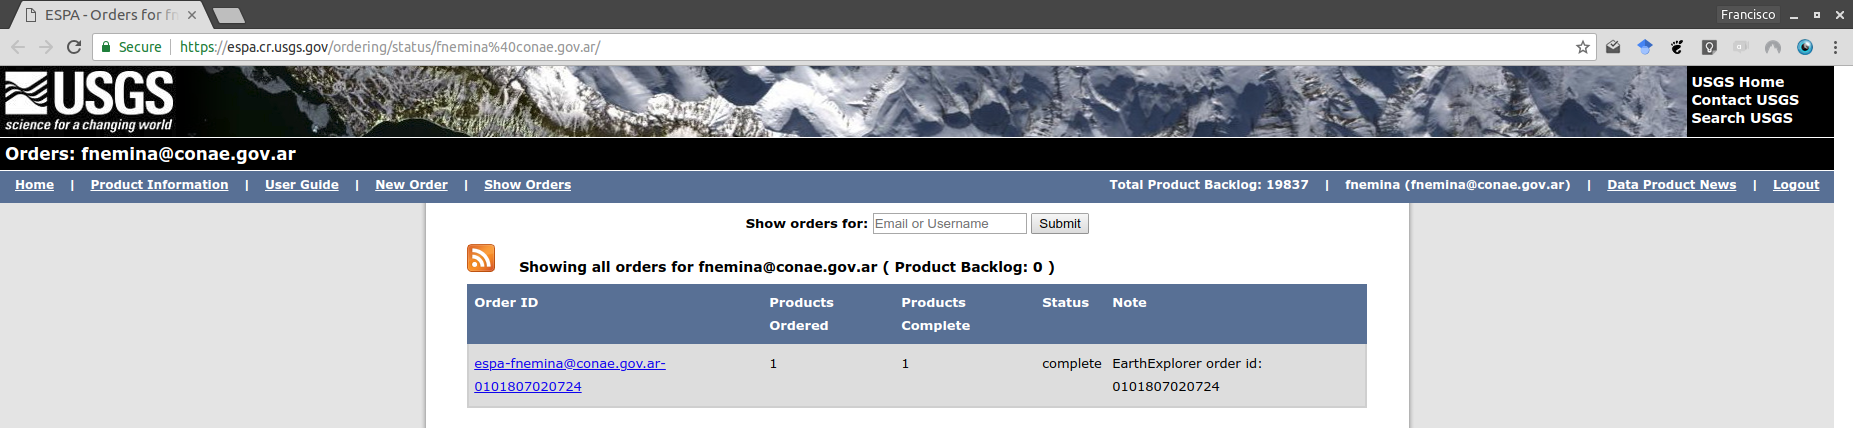
\includegraphics[width=0.6\textwidth]{fig:descarga2.png}}
    \\
    \subfloat[]{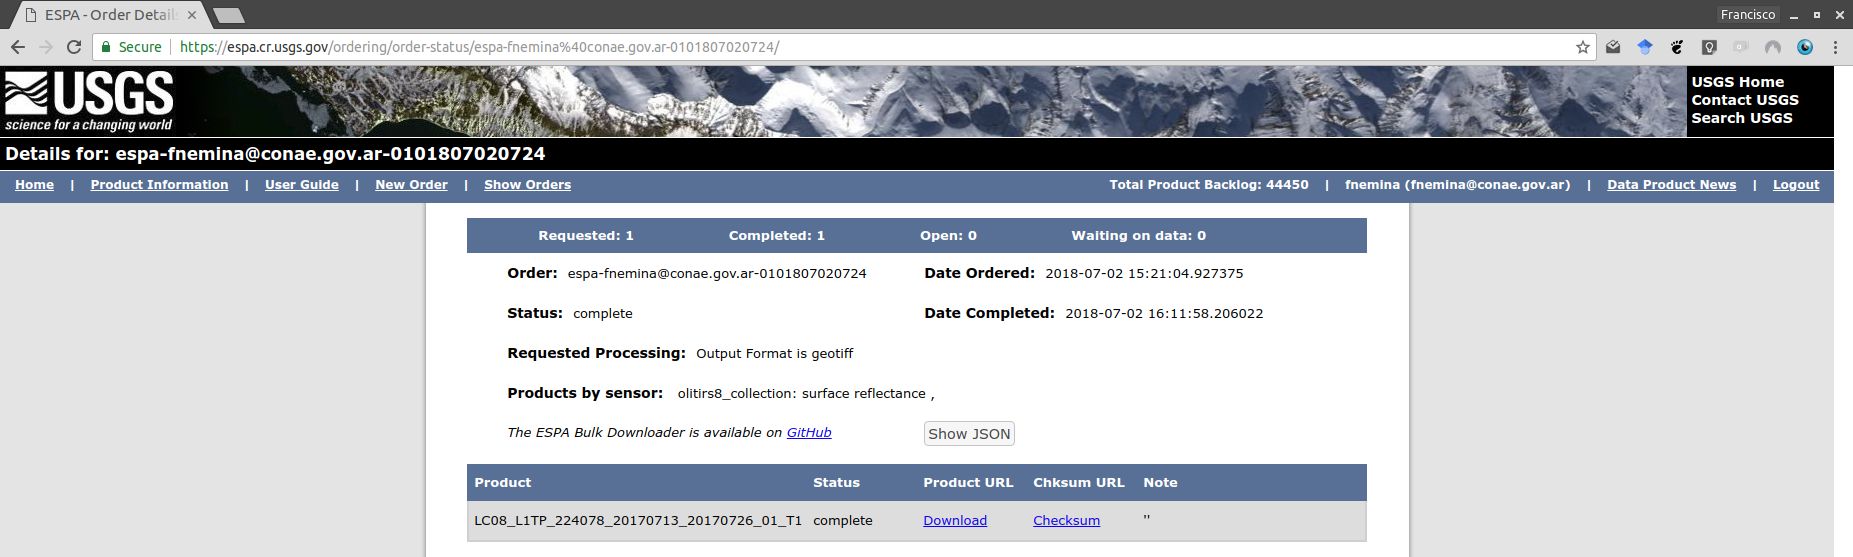
\includegraphics[width=0.6\textwidth]{fig:descarga3.png}}
    \caption{Descarga de productos una vez obtenido el pedido.}
    \label{fig:descarga2}
\end{figure}

\textbf{Observación:} El tiempo para que el producto esté disponible puede ser de hasta 48 horas.

Una vez finalizada la descarga descomprima el archivo. Para ello necesitara un descompresor como winrar, 7zip o similar.

\section{Apilado de bandas}
Dentro de la carpeta descomprimida, las distintas bandas de la imagen se encuentran en archivos separados. Abra en el SNAP los archivos

\begin{center} \directory{LC08\_L1TP\_224078\_20170713\_20170726\_01\_T1\_sr\_band1},
\end{center}
\begin{center} \directory{LC08\_L1TP\_224078\_20170713\_20170726\_01\_T1\_sr\_band2},
\end{center}
\begin{center} \directory{LC08\_L1TP\_224078\_20170713\_20170726\_01\_T1\_sr\_band3},
\end{center}
\begin{center} \directory{LC08\_L1TP\_224078\_20170713\_20170726\_01\_T1\_sr\_band4},
\end{center}
\begin{center} \directory{LC08\_L1TP\_224078\_20170713\_20170726\_01\_T1\_sr\_band5},
\end{center}
\begin{center} \directory{LC08\_L1TP\_224078\_20170713\_20170726\_01\_T1\_sr\_band6}
\end{center}
\begin{center} y \directory{LC08\_L1TP\_224078\_20170713\_20170726\_01\_T1\_sr\_band7}.
\end{center}

Aparecerán en el \emph{Product explorer} a la derecha y podrá visualizar las bandas por separado.

Vaya a \menu{Radar > Coregistration > Stack tools > Create Stack} y en la pestañá \menu{1-ProductSet-Reader} haga click en \menu{Add oppened}. Usando los botones \menu{Move up} y \menu{Move down} ordene las bandas según su nombre (Figura \ref{fig:stack1}).

En la pestaña \menu{2-CreateStack} seleccione la opción \emph{Product Geolocation} para el parámetro \menu{Initial Offset method} (Figura \ref{fig:stack2}).

Finalmente en la pestaña \menu{3-Write} elija el nombre del archivo de salida y la carpeta donde se guardarán los datos. Haga luego click en \menu{Run}. El resultado se agregará al \emph{Product explorer}(Figura \ref{fig:stack3}).

\begin{figure}[h!]
    \centering
    \subfloat[1-ProductSet-Reader]{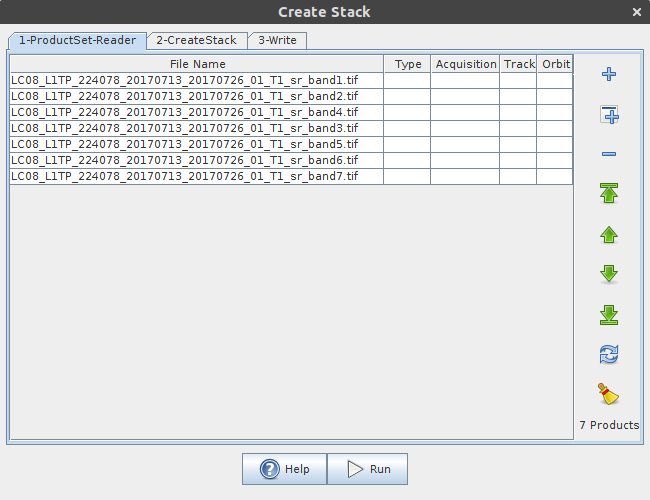
\includegraphics[width=0.4\textwidth]{fig:stack1.png}\label{fig:stack1}}
    \hspace{1cm}
    \subfloat[2-CreateStack]{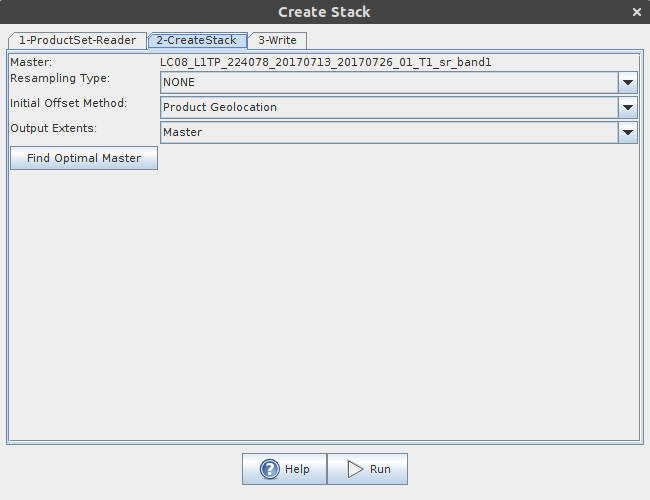
\includegraphics[width=0.4\textwidth]{fig:stack2.png}\label{fig:stack2}}\\
    \subfloat[3-Write]{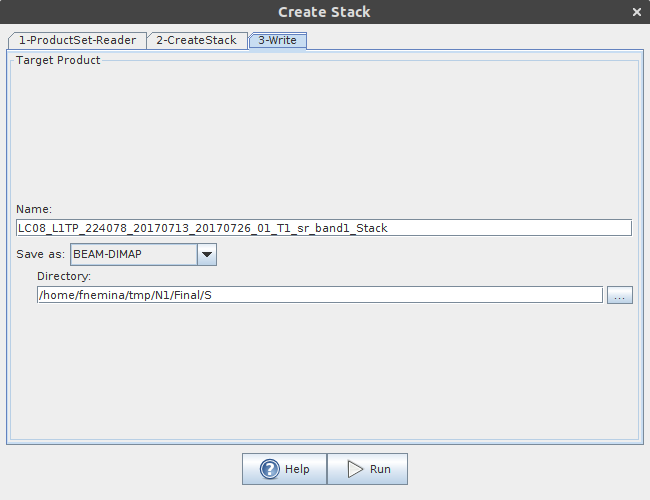
\includegraphics[width=0.4\textwidth]{fig:stack3.png}\label{fig:stack3}}
    \caption{Apilado de productos en el SNAP usando la herramienta \menu{Create Stack}.}

\end{figure}

\section{Propiedades de la imagen}
Es de utilidad editar las propiedades de la imagen para agregar los nombres de las bandas, su longitud de onda central y tipo de dato.

En la sección de bandas de la imagen creada, haga click derecho sobre
\begin{center}
\texttt{band\_1\_mst\_01Jan2000}
\end{center}
y luego seleccione \menu{Properties}. En al ventana que se despliega es posible cambiar el nombre de la banda, la unidad en la que está medida, el valor digital no valido, la longitud de onda central de la banda y su ancho (Figura \ref{fig:prop}).

\begin{figure}[h!]
    \centering
    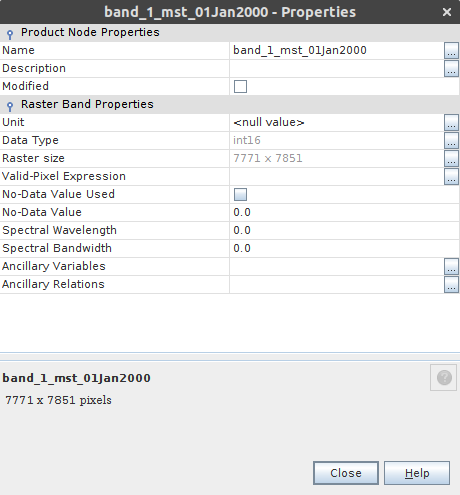
\includegraphics[width=0.35\textwidth]{fig:prop.png}
    \caption{Propiedades de una banda de la imagen. Se observan los valores de nombre y longitud de onda, entre otros.}
    \label{fig:prop}
\end{figure}

Edite los campos \emph{Name} con el valor \texttt{ca} y el campo \emph{Spectral Wavelength} con el valor \texttt{442}. Repita el proceso para el resto de las bandas (Tabla \ref{tab:landsat8}).

\begin{table}[h!]
  \centering
  \begin{tabular}{@{}lclc@{}}
  \toprule
  Bands designation          & Número & Name  & Wavelength {[}nm{]} \\ \midrule
  Aerosoles costeros         & 1      & ca    & 442                 \\
  Azul                       & 2      & blue  & 482                 \\
  Verde                      & 3      & green & 561                 \\
  Rojo                       & 4      & red   & 655                 \\
  Infrarrojo cercano         & 5      & nir   & 865                 \\
  Infrarrojo de onda corta 1 & 6      & swir1 & 1610                \\
  Infrarrojo de onda corta 2 & 7      & swir2 & 2200                \\ \bottomrule
  \end{tabular}
\caption{Nombres de las bandas y longitudes de onda para el producto Landsat 8 - level 2 collection.}
\label{tab:landsat8}
\end{table}

Para guardar los cambios realizados en la imagen haga click derecho sobre ella y elija \menu{Save product}.

\section{Subset espacial y espectral}
Para trabajar solo con nuestra región de interés reduciendo el tamaño de la imagen y por
lo tanto los tiempos de procesamiento, es posible hacer un recorte o subset, tanto espacial como espectral, de la imagen.

Para hacerlo, seleccione la imagen apilada y diríjase a \menu{Raster > Subset}. En la pestaña \menu{Spatial subset} seleccione la pestaña \menu{Geo Coordinates} (Figura \ref{fig:subset}).

\begin{figure}[h!]
    \centering
    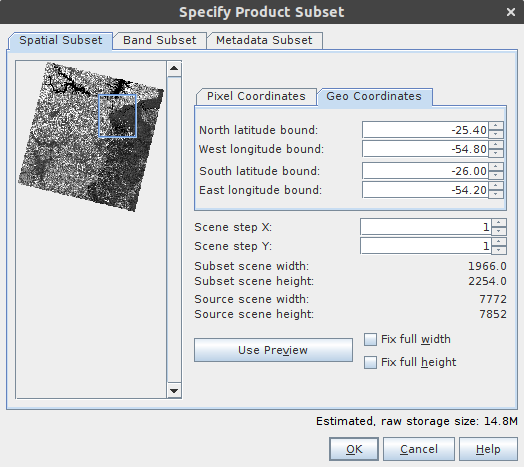
\includegraphics[width=0.45\textwidth]{fig:subset.png}
    \caption{Subset espacial de una imagen Landsat 8 por coordenadas geográficas.}
    \label{fig:subset}
\end{figure}

Haga un recorte introduciendo las coordenadas geográficas

\begin{itemize}
    \item North latitude bound: -25.4
    \item West longitude bound: -54.8
    \item South latitude bound: -26.0
    \item East longitude bound: -54.2
\end{itemize}

y haciendo click en \menu{Ok}.

Es posible también hacer un subset de bandas eligiéndolas de la pestaña \menu{Band subset}.

\section{Reproyección}
Para algunas aplicaciones la proyección por defecto de la imagen puede no ser la más indicada. Para cambiar la proyección diríjase a \menu{Raster > Geometric operations > Reprojection} (Figura \ref{fig:repro}).

\begin{figure}[h!]
    \centering
    \subfloat[I/O Parameters]{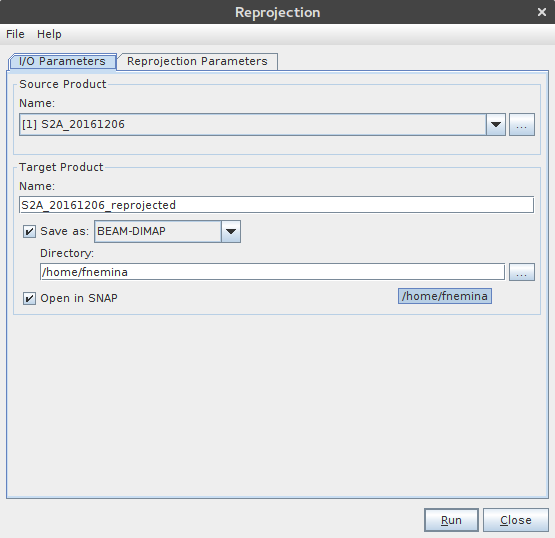
\includegraphics[width=0.4\textwidth]{fig:reproj1.png}}
    \hspace{1cm}
    \subfloat[Processing parameters]{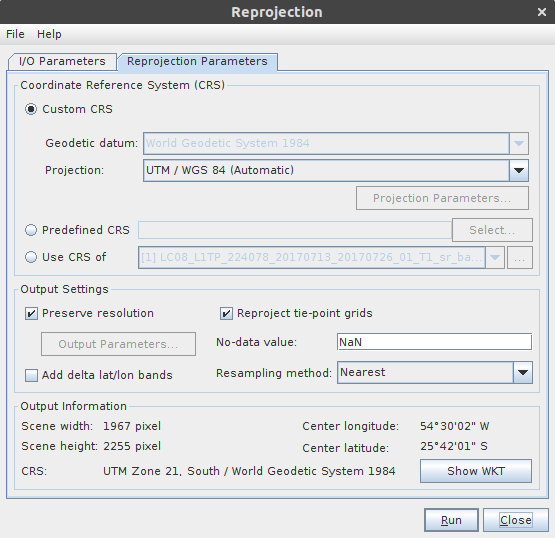
\includegraphics[width=0.4\textwidth]{fig:reproj2.png}}
    \caption{Herramienta de reproyección del SNAP. La imagen se proyecta en coordenadas geográficas.}
    \label{fig:repro}
\end{figure}

Seleccione en la pestaña \menu{I/O parameters} la imagen recortada como imagen de entrada. Puede aquí seleccionar el nombre y la carpeta del archivo de salida. Utilice el nombre

\begin{center}
  \directory{LC08\_224-078\_2017-07-13.dim}
\end{center}

En la pestaña \menu{Reprojection parameters} elija la opción \emph{Custom CRS} y allí del menú desplegable seleccione \emph{UTM / WGS 84 (automatic)}. De esta forma la imagen será reproyectada a la faja correspondiente del sistema de coordenadas \emph{UTM/WGS84}. Haga click en \menu{Run}.

\section{Actividad práctica}

\begin{enumerate}
  \item Identifique en la imagen descargada los siguientes objetos:
  \begin{enumerate}
    \item El río Iguazú que recorre la imagen de izquierda a derecha en color gris/marron.
    \item El río Paraná que corta la imagen de arriba a abajo celestre.
    \item La ciudad de Puerto Iguazú al sur-este del cruce de los rios Iguazú y Paraná.
    \item La zonas cultivadas al norte del río Iguazú con formas de parches en color verde.
    \item Laz onas cultivadas al oeste del río Paraná formadas por parches de color verde, con cultivo, y rosa, sin cultivo.
    \item La selva Paranaense al sur del río Iguazú en color verde.
    \item El embalse Urugua-í al sur de la imagen.
    \item La zona de forestaciones en color verde más oscuro entre la selva Paranaense y el embalse Urugua-í.
    \item El aeropuerto de cataratas del Iguazú en medio de la selva Paranaense.
  \end{enumerate}
  ¿Que combinación de bandas conviene utilizar para identificar cada uno?

  \item Objenga una firma espectral de:
  \begin{enumerate}
    \item El río Iguazú.
    \item El río Paraná.
    \item El embalse Urugua-í.
    \item La selva paranaense.
    \item Una forestación.
    \item Suelo con cultivo.
    \item Suelo en descanso.
  \end{enumerate}

  \item Compare visualmente la imagen Landsat 8 del 5 de enero de 2018 y del 13 de julio de 2017. Elija la combinación de bandas que considere adecuada.
  \begin{enumerate}
    \item Que observa sobre el río Paraná e Iguazú.
    \item Que observa sobre la selva paranaense.
    \item Que observa en la zona de forestaciones.
    \item Que observa en la zona de cultivos.
  \end{enumerate}
  ¿En que se parecen? ¿Que coberturas cambian de color entre las dos imágenes?

  \item Compare las firmas espectrales obtenidas de la imagen Landsat 8 del 5 de enero de 2018 y del 13 de julio de 2017.
  \begin{enumerate}
    \item Sobre el río Paraná.
    \item Sobre el río Iguazú.
    \item Sobre la selva Paranaense.
    \item Sobre las forestaciones.
    \item Sobre un mismo parche de cultivo.
  \end{enumerate}
  ¿Que firmas espectrales cambian más entre las dos imágenes? ¿A que se debe este cambio? ¿Cómo se explica en término de las propiedades biofísicas de la cobertura observada?
\end{enumerate}

Estas preguntas y actividades no serán evaluadas. Su objetivo es discutirlas en el foro de consultas e intercambio de la clase.
